\documentclass[a4paper,10pt]{paper}
%\documentclass[a4paper,10pt]{scrartcl}

\usepackage[latin9]{inputenc}
\usepackage{ae}
\usepackage{marvosym}
\usepackage{multirow}
\usepackage[ngerman,english]{babel}
\usepackage[T1]{fontenc}
\usepackage{graphicx}
\usepackage{datetime}



%\title{\Large Lab Exercise:\\Implementing an OFDM Receiver by Software Defined Radio}
%\date{\today}

\pdfinfo{%
    /Title    ()
        /Author   ()
        /Creator  ()
        /Producer ()
        /Subject  ()
        /Keywords ()
}

\begin{document}
\begin{titlepage}
{
\centering
{\Huge Lab Exercises}\\[15mm]
{\Large \textbf{Modules:}}\\[3mm]
{\Large Communications Engineering}\\[1mm]
{\Large and}\\[1mm] 
{\Large Computer Engineering}\\[20mm]
{\huge \textbf{Experiment at 
\includegraphics[height=16pt]{ti_veclogo}} :}\\[5mm]
{\huge \textsc{Implementing an OFDM}}\\[2mm]
{\huge \textsc{Transceiver by}}\\[2mm]
{\huge \textsc{Software Defined Radio}}\\[8mm]

{\textbf{Location}: Seminar room 332, ICT cubes, Kopernikusstra{\ss}e 16, 52074 Aachen, at TI}\\[2mm]
{\textbf{Contact}: \texttt{laboratory\MVAt ti.rwth-aachen.de}}\\[30mm]

{\Large Hostname: \textbf{\input{envar}} }\\[6mm]
{\Large Date: \ddmmyyyydate \today}\\[30mm]
%\hrulefill
%{\huge \textbf{Important remark:}}\\[2mm]
%{\Large As preparatory steps read the experiment description and solve the exercises of Chapter/Section ...}\\[37mm]
%{\Large Before coming to lab, students should read the script and solve the preparatory exercises in Chapter~\ref{ch:preparation}.}\\[30mm]
}

\begin{tabular}{@{}lll@{}}
\multirow{3}{37pt}{
\includegraphics[height=32.3pt]{ti_veclogo}} & Institute for Theoretical & \multirow{3}{37pt}{\hspace*{-4cm}
\includegraphics[height=32.3pt]{RWTHAachenUniversity}}\\
& Information Technology&\\
& Univ.-Prof.~Dr.~rer.~nat.~Rudolf Mathar\phantom{blablablablablablablabl}&
\end{tabular}
\end{titlepage}
\newpage



%\section{Results:}
\section{Task 2}
This exercise is implicitly related to the analytical results obtained in the preparatory exercises. In order to achieve particular BER, each modulation requires a certain SNR value which defines the rate-power function for a given system. BER values of~$10^{-2}$ and~$10^{-3}$ are investigated.
\begin{figure}[h]
\centering
\includegraphics[width=0.64\linewidth]{exercise_11.eps}
\caption{Rate-power functions for RF transmission using the OFDM system with 1~MHz bandwidth, 200 data subcarriers, 256 FFT length}
\end{figure}
\begin{figure}[h]
\centering
\includegraphics[width=0.64\linewidth]{exercise_12.eps}
\caption{Measured BERs}
\end{figure}

\newpage
\section{Task 3}
The goal of this exercise is to demonstrate the bandwidth efficiency of OFDM systems in frequency selective channels. The experiment is based on system simulation since the real channel environment for the given transmission bandwidth does not experience multipath propagation. Firstly, the OFDM system where \textbf{all} subcarriers are loaded with BPSK symbols is simulated. The required BER is reached by fitting the transmit amplitude. Then, using the same transmit amplitude, the OFDM system is simulated using the \textbf{better half} of the subcarriers loaded with QPSK symbols, thus preserving the same data rate and halving the bandwidth usage. This usage of subcarriers per modulation scheme is depicted in Fig.~\ref{fig:FSC}.
\begin{figure}[thb]
\centering
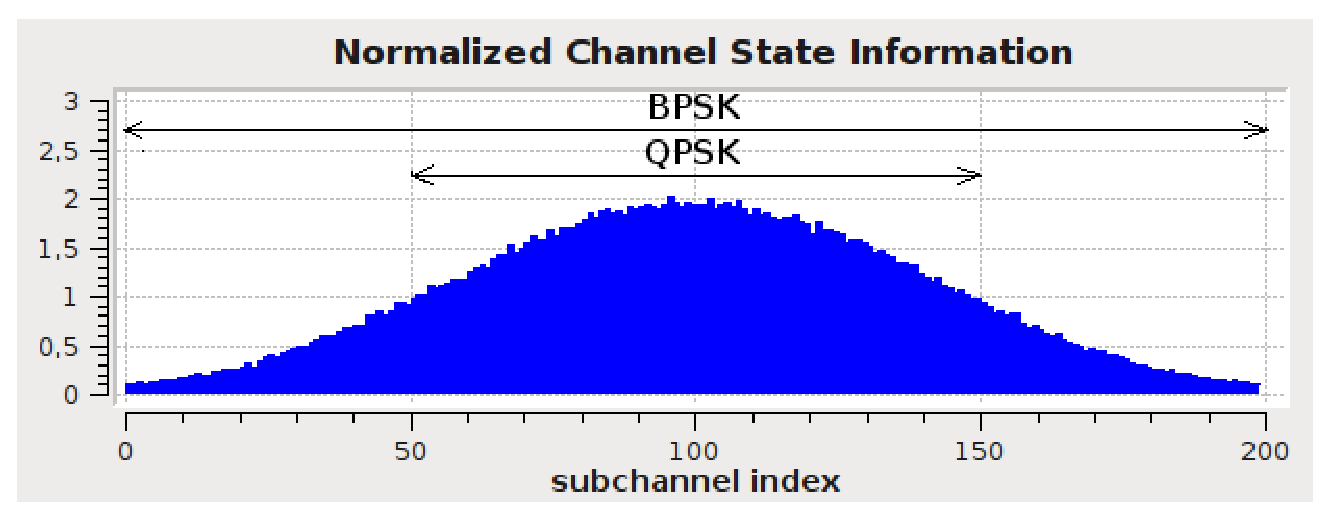
\includegraphics[width=.95\linewidth]{csi.eps}
\caption{Using all subcarriers with BPSK and using the better half with QPSK}\label{fig:FSC}
\end{figure}
\begin{figure}[thb]
\centering
\includegraphics[width=0.76\linewidth]{exercise_2.eps}
\caption{BER for simulated OFDM system in frequency selective channel with 1~MHz bandwidth, 200 data subcarriers, 256 FFT length}
\end{figure}

\newpage
\section{Task 5}
This exercise investigates the influence of frequency offset on system performance. Without loss of generality, the experiment is conducted only for QPSK modulation scheme and performance is depicted jointly with analytical results. 
\begin{figure}[thb]
\centering
\includegraphics[width=1.00\linewidth]{exercise_3.eps}
\caption{SNR loss over frequency offset for different SNRs, analytical and simulation results}
\end{figure}

\end{document}
